\documentclass[nosignatures]{mscThesis}
% replace the previous line with the next to include a signature page
%\documentclass{mscThesis}
% use the option 'nosignatures' to turn off the signatures page
%\documentclass[nosignatures]{mscThesis}
%
% Thesis data
%-For Confidential Reports, uncomment the next line, if desired change the argument. It is printed on the cover, title page and in the footer per page
%\mscConfidential{CONFIDENTIAL}
%
%-Definition of department, programme, faculty
\mscDepartment{Delft Center for Systems and Control (\textsmaller{DCSC})}%
\mscProgram{Systems and Control}
%Change if needed to
%\mscProgram{Mechanical Engineering}
\mscFaculty{Mechanical, Maritime and Materials Engineering (3mE)}%
%
%-name, date, title
\mscName{J. Random Student}%
\mscDate{\today}%
\mscTitle{Thesis Title}%
\mscSubTitle{Optional Subtitle}%
\mscKeyWords{thesis, msc, subject}% only used in PDF properties
%
%-cover picture
\mscCoverPicture{STYLESTUFF/COVER}% to place a picture ( here the example COVER.eps) on the cover page. Comment out if no picture is to be used
%
%
%-Third party options (create text/logo on the copywrite page)
\mscThirdPartyText{The work in this thesis was supported by Aquaduct Swimming Supplies Incorporated. Their cooperation is hereby gratefully acknowledged.}
\mscThirdPartyLogo{STYLESTUFF/EXAMPLELOGO}
% NOTE: on the title page only the TU Delft logo is permitted.
%
%
% The examination committee  - Supervisors and Readers
\mscSupervisorOne{prof.dr.ir.~M.Y.~Supervisor}
\mscSupervisorTwo{Dr.ir.~M.Y.~Second Super}
%\mscSupervisorThree{}
\mscReaderOne{prof.dr.ir.~M.Y.~First Reader}
\mscReaderTwo{dr.ir.~F.S.T.~Reader-two}
\mscReaderThree{ir.~Th.~Reader-three}
%\mscReaderFour{}
%
% Finalize the thesis data
\setThesisInfo
%
% Use \includeonly{} to build only certain parts of your thesis
%\includeonly{introduction, real_chapter, empty_chapter, long_chapter}%
%
%PH Toegevoegd 24-10-2011
%allow (matlab, C++ etc) listing max 1pt flexibility between lines
\lstset{lineskip=0pt plus 1pt minus 0pt} %%
%
\begin{document}
%
%========================== Front matter ======================================
\frontmatter %
%
% Make the cover page and hell of a lot of title pages
\maketitle
%
%
% Abstract (does not appear in the Table of Contents)
\chapter*{Abstract}%

Pedestrian indoor localization is a problem  yet to have a solution that is as generally accepted as the Global Positioning System is for outdoor localization. An infrastructure independent option is to leverage the data from \ac{IMU} sensors to determine position. A large advantage of this approach is that these sensors are already available to many people since they are often integrated in the modern smartphone. Creating an indoor localization solution that works on this device could lead to wide adoption. This has been recognized by the research community, with methods already being tested on the device. An interesting combination worth considering is the combination of smartphone based indoor localization with the emerging market of wearable technology. This new technology has the potential to provide additional information that could improve indoor localization. One option is to detect activity that is not easily detectable from smartphones alone.

Within this thesis, a proof of concept is designed with the goal of finding a way in which activity recognition from wearable tech can help smartphone based indoor localization.
The implementation within this thesis relies only on the \ac{IMU} data of a smartwatch and smartphone, and map information of the indoor environment. It produces a position estimate of a pedestrian within the indoor environment. \par 

The system consists of two subsystems placed in series, where the output of the first subsystem, the \ac{SHS}, is the input of the second subsystem, the Particle Filter with  spatial context. The \ac{SHS} uses \ac{IMU} data from the smartphone to determine if a step is taken, what its length is, and in what direction it was taken. When multiple steps are taken a \ac{SHS} trajectory is generated as output of the subsystem.
The Particle Filter with spatial context uses the \ac{SHS} trajectory to generate position estimate in an indoor environment. It uses spatial constraints, such as walls, to limit the estimate. The \ac{IMU} data of a smartwatch is used to detection door interactions. These interactions in combination with known door locations, calibrates the position estimates to door locations. \par 

In order to evaluate performance, experiments was performed in an indoor environment where map information was available, with 6 trials being walked. Smartphone and smartwatch {IMU} data was recorded. Door interactions were also recorded manually.
Results from the experiments show that activity recognition can improve position estimates, however false positive in the recognition can have a detrimental effect on the position estimate.


%
% table of contents, (\toc of \toclof of \tocloflot )
\tocloflot
%
%
%
% Preface
\chapter{Preface}

According to \textsc{WikipediA}, a preface (pronounced ``\emph{preffus}'') is an introduction to a book written by the author of the book. In this preface I can discuss the interesting story of how this thesis came into being. 

This is document is a part of my Master of Science graduation thesis. The idea of doing my thesis on this subject came after a discussion with my good friends Tweedledum and Tweedledee\ldots




%
% Acknowledgements
\chapter{Acknowledgements}%

\textcolor{red}{Acknowledgements still needs to be written}

%I would like to thank my supervisor \mscreaderone\ for his assistance during the writing of this thesis\ldots
%
%By the way, it might make sense to combine the Preface and the Acknowledgements.  This is just a matter of taste, of course.



\vspace*{15mm}

Delft, University of Technology \hfill \mscname \\
\mscdate
%
% Dedication page. 
\cleardoublepage
\thispagestyle{empty}
\vspace*{\stretch{1}}

% Put your own motto here, or dedicate your work to your Mom or whatever...
\begin{quote}
\noindent``In the future, airplanes will be flown by a dog and a pilot. And the dog's job will be to make sure that if the pilot tries to touch any of the buttons, the dog bites him.''
	
--- \emph{Scott Adams}
\end{quote}

\vspace{\stretch{3}}
\clearemptydoublepage
%
%========================== Main matter ======================================
\mainmatter
%

\chapter{Introduction} \label{chap:intro}

Indoor localization is an ongoing research field where there is yet a solution to be found that is widely accepted as the state of the art \cite{Davidson2017}. For outdoor localization the de facto solution is the Global Positioning System \cite{Jackermeier2018}. The GPS solution can not be applied reliably in an indoor environment, due to the difficulty of the system's radio waves in traversing solid structure and if recieved the possibility of them being rebounded off of surfaces, causing erroneous positioning estimates. As with outdoor localization, indoor localization has a large range of possible applications. Examples include navigation in unknown environments, such as firefighters in an emergency situation or personal navigation through large public buildings, and the tracking of individuals, such as within elderly homes or workers in a factory setting. For wide applicability it is preferable that an indoor localization method has as little dependencies as possible, ensuring that little to no installation is required for it to work. \par 
Indoor localization requires a portable platform on which to perform position estimation. The most obvious platform for this is the smartphone, a device ubiquitous in the developed world. It contains a wide range of different sensors combined with computing capabilities, while being untethered. Creating a system that works well on this device will be crucial to launching indoor localization on a global scale \cite{Gu2019}. Focusing on this platform brings additional restrictions to what any eventual solution can use. This includes carrying modes and computational requirements. \par 
While the smartphone market has matured, the market of wearable devices has been growing steadily \cite{jung2016consumer}, with the smart watch being the most prominent. Similarly to the smartphone, these devices are fused with different sensors gathering information. In addition these devices often have communication capabilities, allowing them transfer and receive information from an external device. This provides a new source of data that can be combined with smartphone based solution to potentially help improve indoor localization. The use of these sensors within localization have not been studied much so far, and deserve further investigation.
%A solution with the potential to meeting the above requirements is Pedestrian Dead Reckoning (PDR), a technique where the displacement from an initial location is calculated for a pedestrian. This technique often uses inertial sensors, with different possible placements on the body \cite{Gu2019}. These sensors are \ac{MEMS}, and consist of triaxial orthogonal accelerometers and gyroscopes, and can include a triaxial magnetometer \cite{Yang2014}. These sensors are small, lightweight and cheap, and are found in almost all smartphone brands.
%While able to generate a position estimate for the pedestrian, position estimation drift is inevitable



%Dead reckoning (DR) presents an interesting, incremen­tal positioning modality for pedestrians, complementary to absolute positioning of modern mobile phones (GPS, WiFi, Bluetooth and others). Many location aware applications can profit from greater accuracy and indoor availability, that can be achieved by combining DR with absolute positioning modalities. While dead reckoning is limited for long-term use due to error accumulation, it can achieve high short- to mid-term accuracy, and can be used to gap non-availability phases ^citation from Dead Reckoning from the Pocket - An Experimental StudyUlrich Steinhoff* and Bernt Schiele*t
 
%Although global positioning system (GPS)–based outdoor localization is very common, indoor localization remains a challenge because GPS signals are unavailable indoors. Many indoor localization methods are based on wireless radio systems, such as Wi-Fi [2], radio-frequency identity [3], ultra-wideband [4], and Bluetooth [5]. These localization methods can be categorized into two types [6]: triangulation and fingerprinting. The former relies on installed expensive hardware, making it neither scalable nor universal. The latter requires pretraining, which is time-consuming. citation from A Robust Step Detection and Stride Length Estimation for Pedestrian Dead Reckoning Using a Smartphone 


%Repurposing smartphones for ubiquitous sensing is challenging due to their battery constraints and multi-purpose nature. We observed that each embedded sensor has a similar power draw if used individually, but using combinations of sensors costs significantly more (see Figure 1). Thus, we use solely the accelerometer (applicable even to early smartphones). Smartphones are not dedicated sensing devices and they suffer from dropped samples and significant jitter in signal timestamps. Moreover, their nonrigid attachment (they may be carried in front pockets; back pockets; shirt pockets; hands; bags and more) and freedom of motion violate many of the assumptions made in previous step detection work. citation from Brajdic and harle 2013 


\section{Research Questions}

In order to tackle the subject, two main research question can be defined, with further explanation below them.

\begin{itemize}
	\item \textbf{How can indoor localization be achieved with realistic smartphone placement, while taking computation capabilities into account?}
	\item\textbf{How can wearable devices improve the above derived method?}
\end{itemize}

\section{Thesis Contributions}
This thesis will explore the different possibilities for realistic smartphone based indoor localization and how wearable devices can aid in improving a position estimate. It will explore a proof of concept with the intention of showing the increased performance when data from wearable technology is available. This thesis will test the designed system's performance in experiments, highlight the different advantages, disadvantage and limitations. Future steps are outlined on how to improve the derived method for future research.

\section{Thesis Outline}
%
% A Real Chapter
\chapter{First Real Chapter}

This is real chapter for \ac{DCSC}, ok? We will use it as a demo for the different headings you can use to structure your text.


\section{First Section}

This is the section. Referring to equations, figures and tables can easily be done by the commands \verb"\eqnref{}", \verb"\figref{}" and \verb"\tabref{}".

\begin{equation}\label{eq:First}
	H(s) = \frac{1}{s+2}
\end{equation}

You see? Refer to equations like this \eqnref{eq:First}.


\subsection{The first subsection}

Subsections are the last type of sectioning that is numbered. 


\subsubsection[Subsection Short Title]{The first sub-subsection with a very very very long title, but in the Table of Contents one can only see the short title}

Quick! Check the Table of Contents! Nice, ain't it?\index{Nice}


\paragraph{A paragraph title}

Subdividing your text in sections and paragraphs automatically makes it nice and structured.
%
% Second chapter
\chapter{Some Basics}

This chapter will cover figures and math. 

\section{Figures}

Figures are constructed using the \texttt{figure} environment:
\begin{verbatim}
\begin{figure}
	\centering
	\includegraphics[options]{imagefile_location}
	\caption{Captions}
	\label{fig:dummy}
\end{figure}
\end{verbatim}

\LaTeX\ automatically decides the best placement of the Figure in your document. This will usually be at the top or bottom of the current page, or at the top of the next page. This system gives good results most of the time, but it can get confused when you have a large number of figures. The command \verb"\clearpage" creates an empty page where any `lost' figures will be printed.

You can refer to a Figure by its label: \verb"\figref{label}". See for instance \figref{fig:dummy}.

\begin{figure}
	\centering
	
\includegraphics[width=0.31415\textwidth]{STYLESTUFF/DCSC}
	\caption{The \acs{DCSC} logo. Pretty nice, eh?}
	\label{fig:dummy}
\end{figure}

\section{Math: \texorpdfstring{$e^{j \pi}=0$}{``Euler's identity''}}

I put some fancy math in the section title. Usually this generates complaints from the \texttt{hyperref} package, because the bookmarks you see on the left can only handle `regular text'. Fortunately, this problem can be solved by using a special command that inserts `regular text' whenever this is necessary during compilation of your thesis: \verb"\texorpdfstring{math}{text}".

For further information about math in \LaTeX, I recommend looking at the Short Math Guide found at \href{http://www.ams.org/tex/amslatex.html}{the website} of the \ac{AMS}. \index{math}

\begin{eqnarray}
% \nonumber to remove numbering (before each equation)
  1 &=& 2\\
  x &=& 5 \\
  y &=& \theta
\end{eqnarray}


\section{More About Acronyms}

After the start of a new chapter all acronyms are reset and are printed as a full acronym the first time it is used again, e.g.\ \ac{DCSC}. After the first use, only the short acronym is printed again: \ac{DCSC}.


\section{More About Nomenclature}

This is a test for nomenclature \lsymb{$A(s)$}{Answer function} \index{test}


%
%
%========================== Appendices =======================================
\appendix
%
%
% An Appendix
\chapter{Indoor Localization Experiment}
\label{appendix:shs_experiment}
\textbf{Apparatus}:

\emph{Hardware}:

\begin{itemize}
	\item
	3 Smartphones
	
	\begin{itemize}
		\tightlist
		\item
		Samsung j5 for video recording
		\item
		Iphone for backup orientation estimation and post processing time
		synchronization
		\item
		One Plus Nord for primary orientation estimation and ground truth
		activity recorder
	\end{itemize}
	\item
	1 apple smartwatch
	\item
	Shirt with two breast pockets
	\item
	Indoor test location
\end{itemize}

\emph{Software}:

\begin{itemize}
	\tightlist
	\item
	Iphone and apple watch app
	(\url{https://apps.apple.com/us/app/sensorlog/id388014573\#?platform=appleWatch})
	\item
	Android app for primary sensor recording
	(\url{https://play.google.com/store/apps/details?id=fr.inria.tyrex.senslogs\&hl=en\&gl=US}
	)
\end{itemize}

\textbf{Calibration}:

Calibrate primary estimation sensor (One Plus Nord) just before
experiment, and perform all calibration at the same location within test
location!

\begin{itemize}
	\item
	\emph{Magnetometer}:
	
	\begin{itemize}
		\tightlist
		\item
		Stand away from any clear magnetic disturbance 
		\item
		rotate the phone in as many orientations as possible, infinity sign
		is often used
	\end{itemize}
	\item
	\emph{Accelerometer}:
	
	\begin{itemize}
		\tightlist
		\item
		Rotate the phone slowly in as many orientations as possible in
		attempting to be in as many orientations as possible.
	\end{itemize}
	\item
	\emph{Gyroscope / Magnetic North / Noise}
	
	\begin{itemize}
		\item
		Lay the phone horizontally and start recording while stationary
	\end{itemize}
\end{itemize}

\textbf{Preparation}:

\begin{enumerate}
	\def\labelenumi{\arabic{enumi}.}
	\tightlist
	\item
	Calibrate One Plus Nord with the calibration method outlined above
	\item
	Determine with which hand you will hold the phone, strap the
	smartwatch to the other hand
	\item
	Ensure that all doors in test location are closed
	\item
	Define start location within test location and record it
\end{enumerate}

\textbf{Testing}:

For \emph{each test run} perform the following steps:

\begin{enumerate}
	\def\labelenumi{\arabic{enumi}.}
	\tightlist
	\item
	Go to start location
	\item
	Start sensor recording on smartwatch and iPhone
	\item
	place iPhone in one of the breast pockets of the shirt
	\item
	Start a video recording on the Samsung phone and place it in the other
	breast pocket, making sure that the lens is not covered and can see
	what is in front of the torso of the test subject, hence also what
	direction is being moved in.
	\item
	Start sensor recording on One Plus Nord, logging the uncalibrated
	accelerometer, gyroscope, and magnetometer. Also record the rotation
	vector that the phone records. This is shown in illustration 1.
	\item
	Walk around test location as naturally as possible, holding the One
	Plus Nord in front of you with the screen point up. Try and keep this
	phone orientation as best as possible.
	\item
	Walk to doors and open them using the arm that has the smartwatch on
	it. When touching a door handle click the button in the android app
	that records the time stamp as shown in illustration 2. Close the door
	behind you, so that it can potentially be opened again later.
	\item
	After walking for around 3 minutes, return to start location
	\item
	Stop recording of sensor and video on all devices
	\item
	export the data (film and sensor) from all 3 devices to the same
	folder, making it clear which trail it was
\end{enumerate}

\textbf{Pictures}:
\begin{figure}[H]
	\centering
	\begin{subfigure}[t]{.45\textwidth}
		\centering
		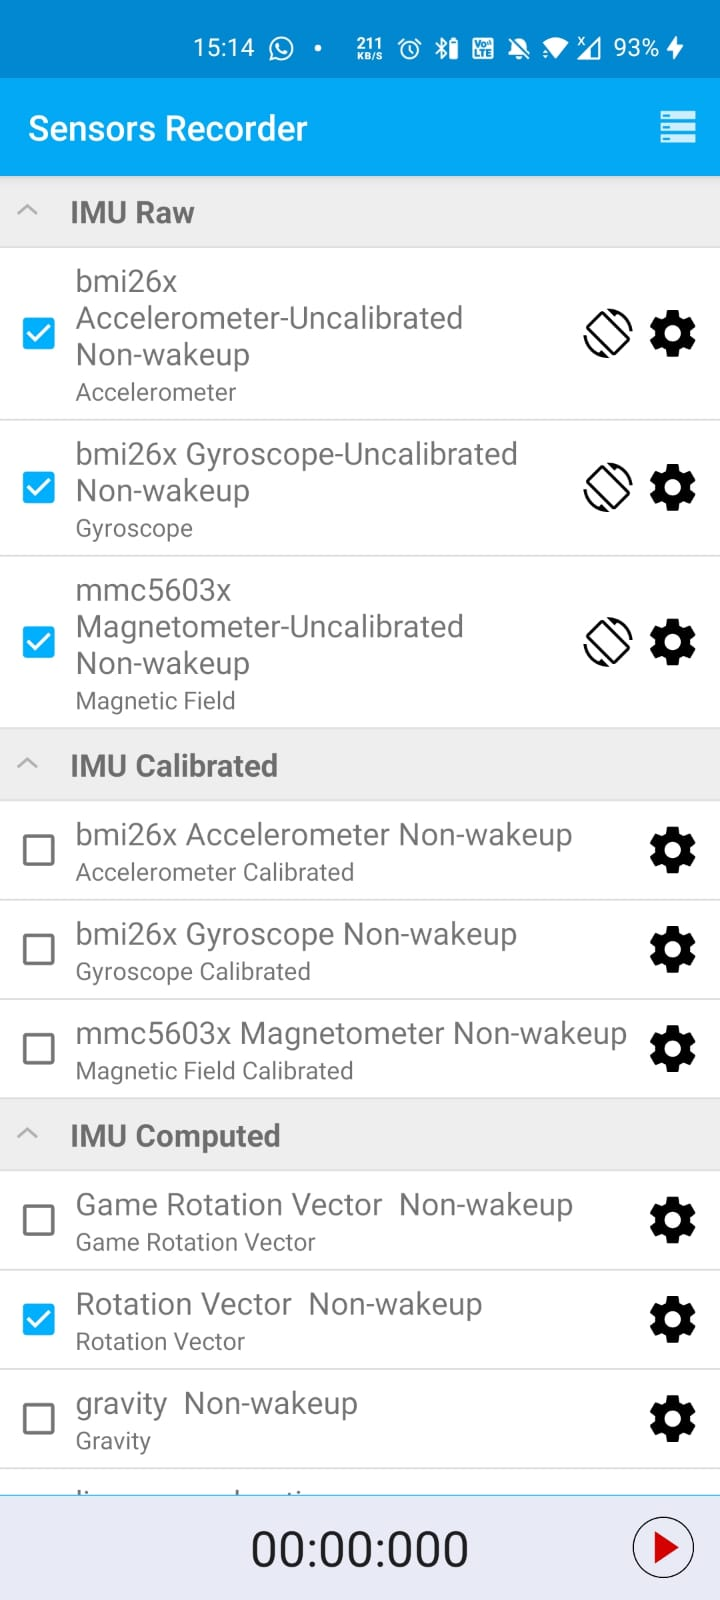
\includegraphics[width=0.6\linewidth]{images/recording_setting}
		\caption{Recording settings}
		\label{fig:recording_setting}
	\end{subfigure}
	\begin{subfigure}[t]{.45\textwidth}
		\centering
		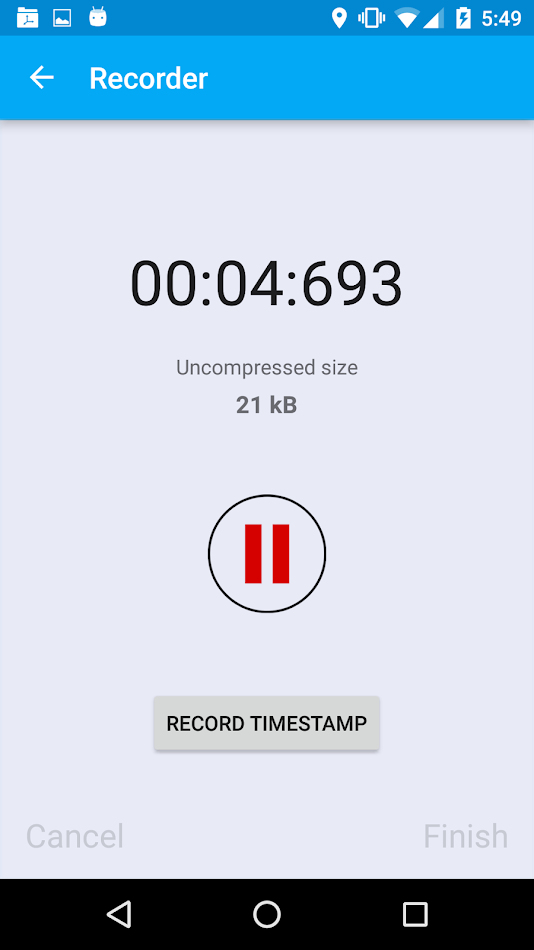
\includegraphics[width=0.7\linewidth]{images/recording_timestamp_button}
		\caption{Record timestamp button}
		\label{fig:recording_timestamp_button}
	\end{subfigure}
\caption{Indoor experiment android app configuration and button}
\end{figure}


\textbf{Postprocessing}

\begin{enumerate}
	\def\labelenumi{\arabic{enumi}.}
	\tightlist
	\item
	Calibrate walking around imu sensor data using calibration data
	\item
	Run calibrated walking around data through orientation estimation
	algorithm
	\item
	Compare result with orientation estimation made by the system and
	maybe even with the iphone 
	\item
	Determine steps and subsequent step length 
	\item
	Combine orientation information and step information to generate an
	estimated trajectory
	\item
	Use this estimated trajectory as input for the particle filter
	\item
	Using the video recording made during testing, manually indicate per
	step where on the blueprint you are. This will be used to determine
	the performance of the estimate of the SHS system. 
\end{enumerate}

\chapter{Indoor Experiment Results}

\section{SHS-PF parameter search}
\begin{figure}[H]
	\centering
	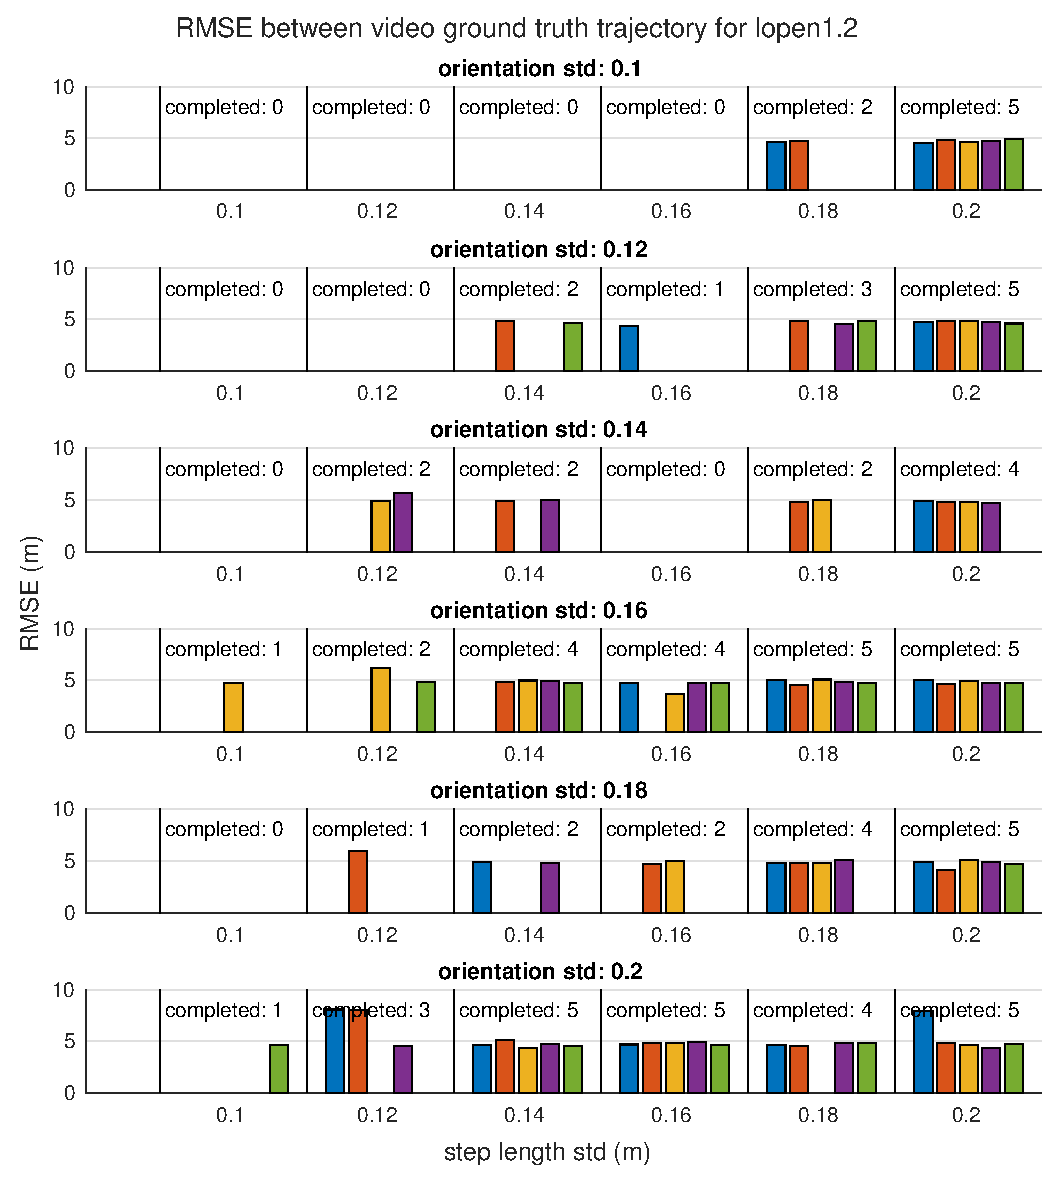
\includegraphics[width=0.7\linewidth]{images/20201107_1312_orientation_std_0_2}
	\caption{}
	\label{fig:202011071312orientationstd02}
\end{figure}
\begin{figure}[H]
	\centering
	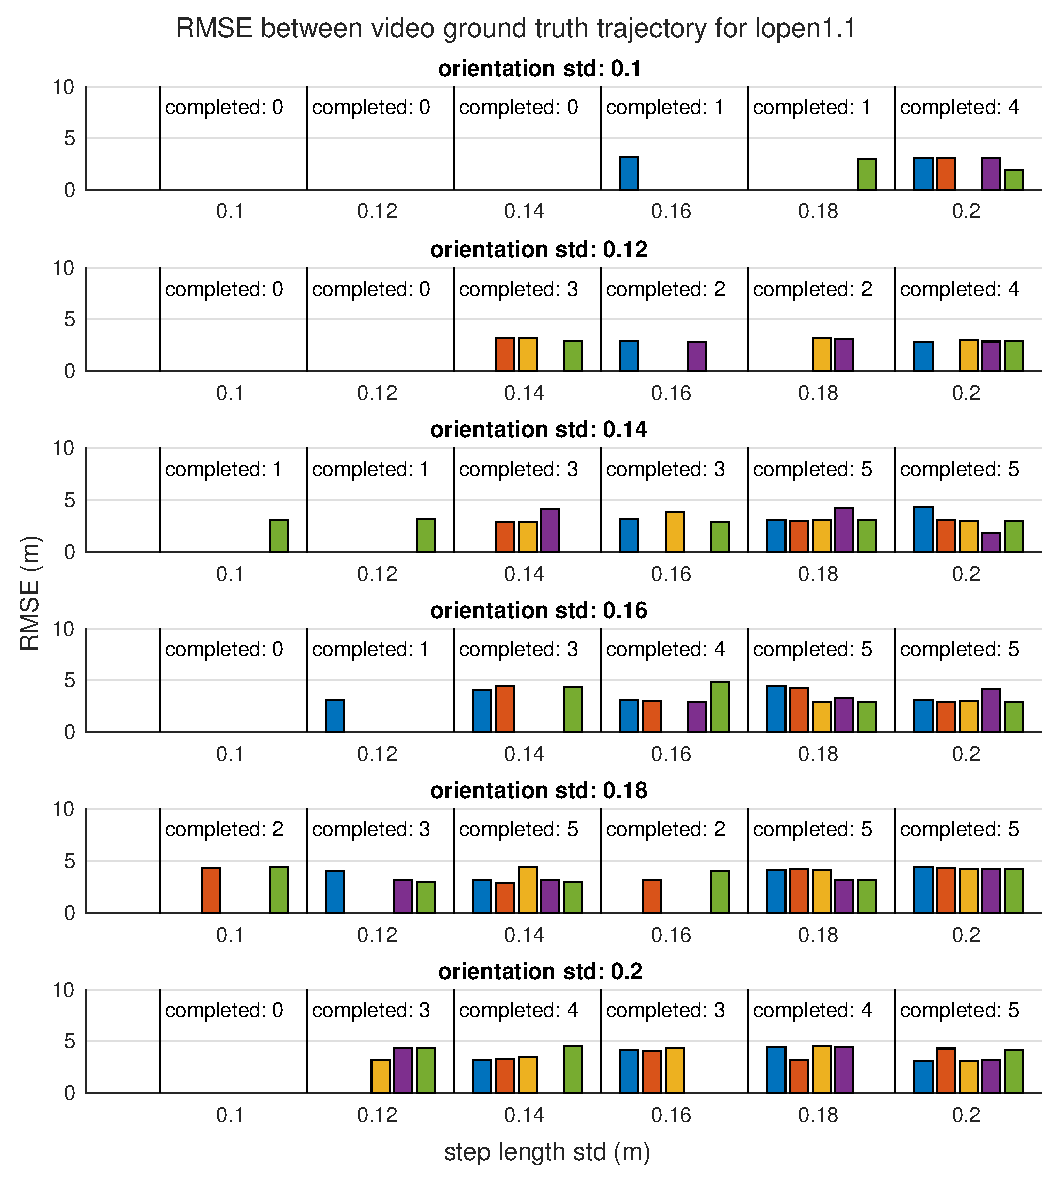
\includegraphics[width=0.7\linewidth]{images/20201107_1311_orientation_std_0_2}
	\caption{}
	\label{fig:202011071311orientationstd02}
\end{figure}

\section{SHS-PF estimator comparison}
\begin{figure}[H]
	\centering
	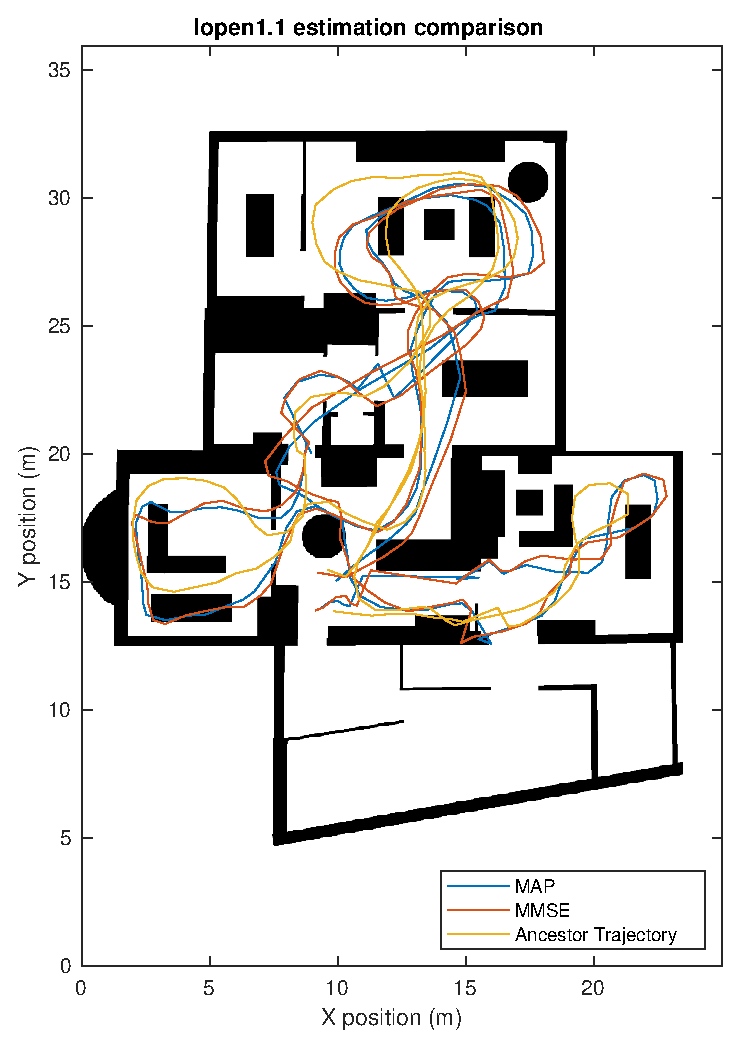
\includegraphics[width=0.5\linewidth]{images/20201108_1559_lopen1_1_estimation_comparison}
	\caption{}
	\label{fig:202011081559lopen11estimationcomparison}
\end{figure}
\begin{figure}[H]
	\centering
	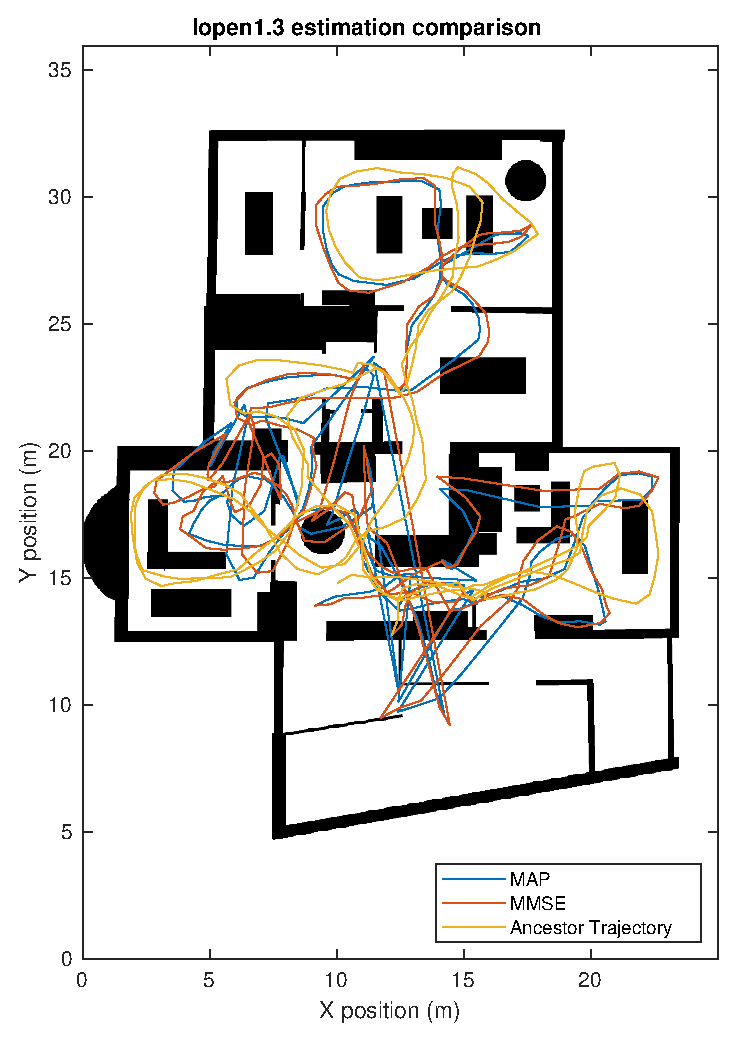
\includegraphics[width=0.5\linewidth]{images/20201108_1601_lopen1_3_estimation_comparison}
	\caption{}
	\label{fig:202011081601lopen13estimationcomparison}
\end{figure}
\begin{figure}[H]
	\centering
	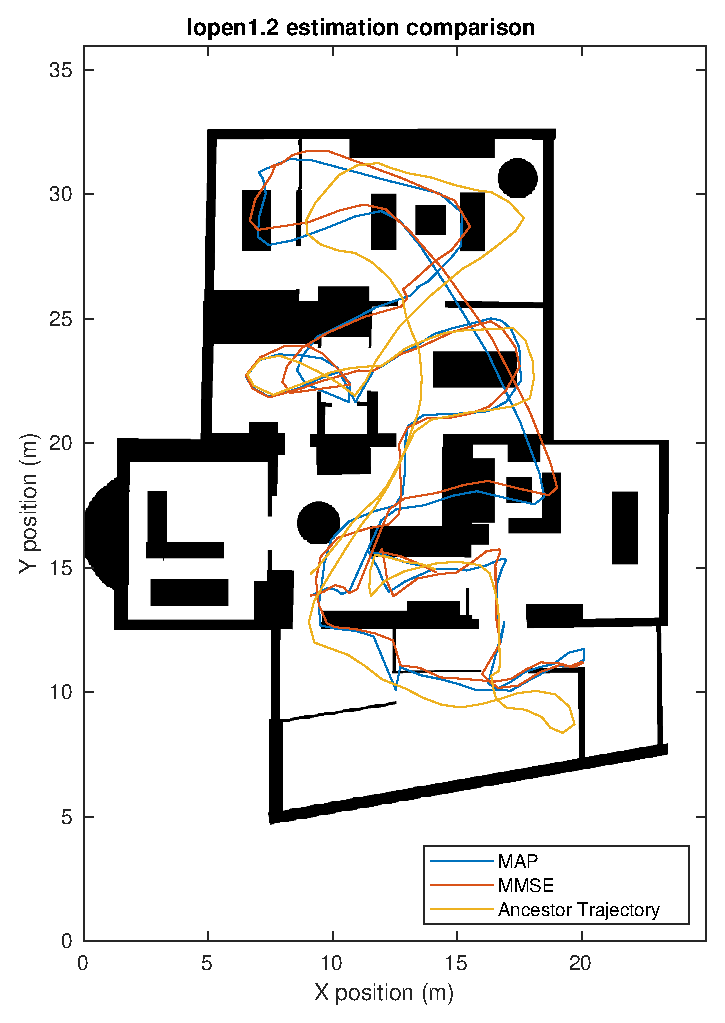
\includegraphics[width=0.5\linewidth]{images/20201108_1559_lopen1_2_estimation_comparison}
	\caption{}
	\label{fig:202011081559lopen12estimationcomparison}
\end{figure}




\section{SHS-PF performance}
\label{app:SHS-PF trials}




\chapter{Experiment trials visualization}
\subsection{Perfect activity recognition}
\newpage
\subsubsection{Trial 1}

\begin{figure}[H]
	\centering
	\begin{subfigure}[t]{.45\textwidth}
		\centering
		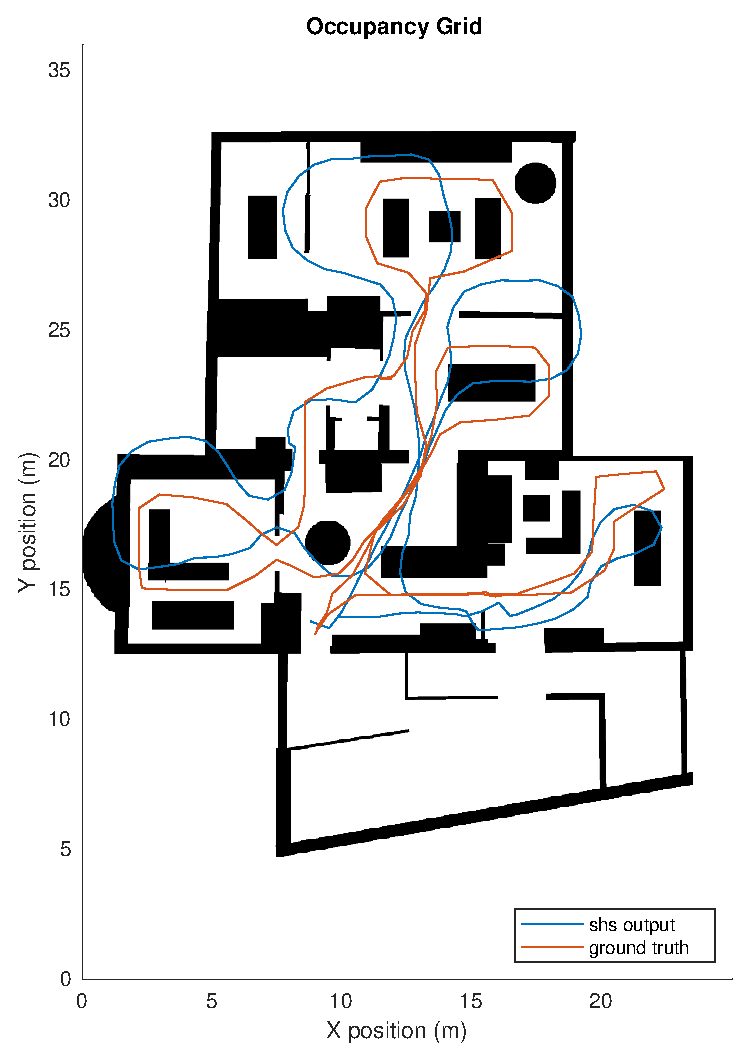
\includegraphics[width=0.9\linewidth]{images/20201029_1040_trial1_shs_1}
		\caption{trajectory comparison}
		\label{fig:trial1_on_map}
	\end{subfigure}
	\begin{subfigure}[t]{.45\textwidth}
		\centering
		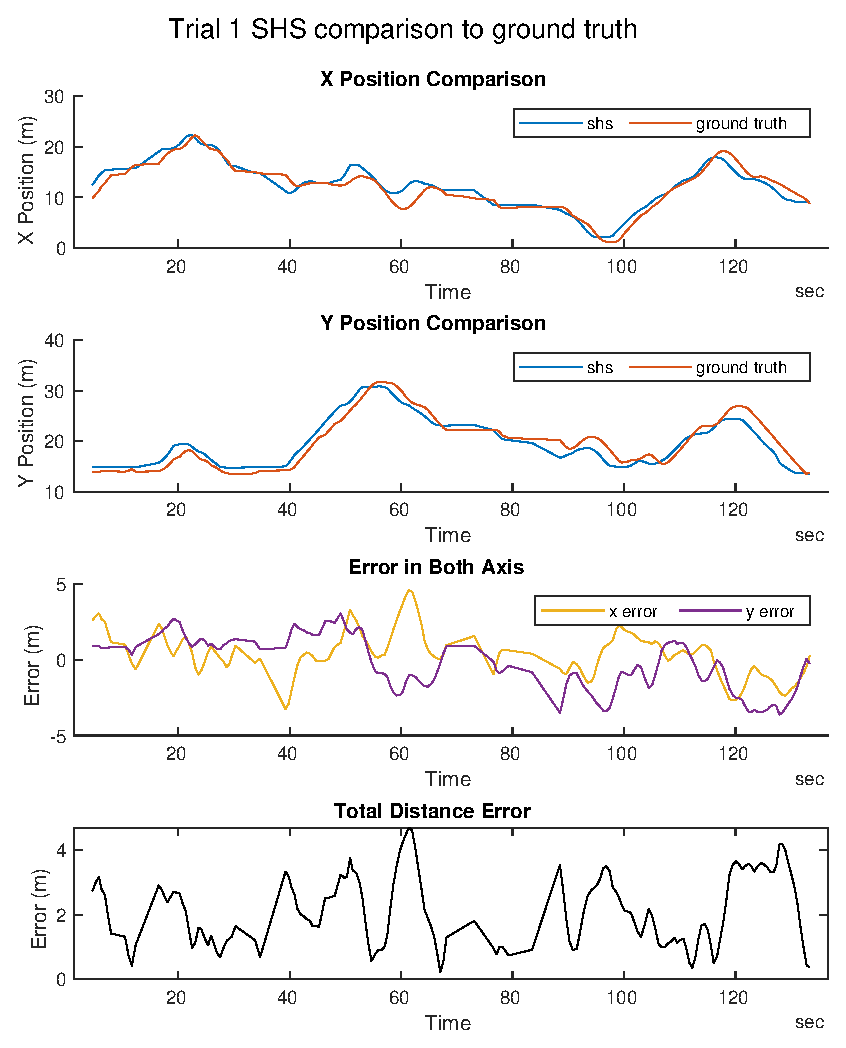
\includegraphics[width=\linewidth]{images/20201029_1040_trial1_shs_2}
		\caption{axis comparison}
		\label{fig:trial1_comparison}
	\end{subfigure}
	\caption{Qualitative SHS comparison of trial 1 with ground truth}
	\label{fig:trial1_shs_gt_comparison}
\end{figure}

\subsubsection{Trial 2}

\begin{figure}[H]
	\centering
	\begin{subfigure}[t]{.45\textwidth}
		\centering
		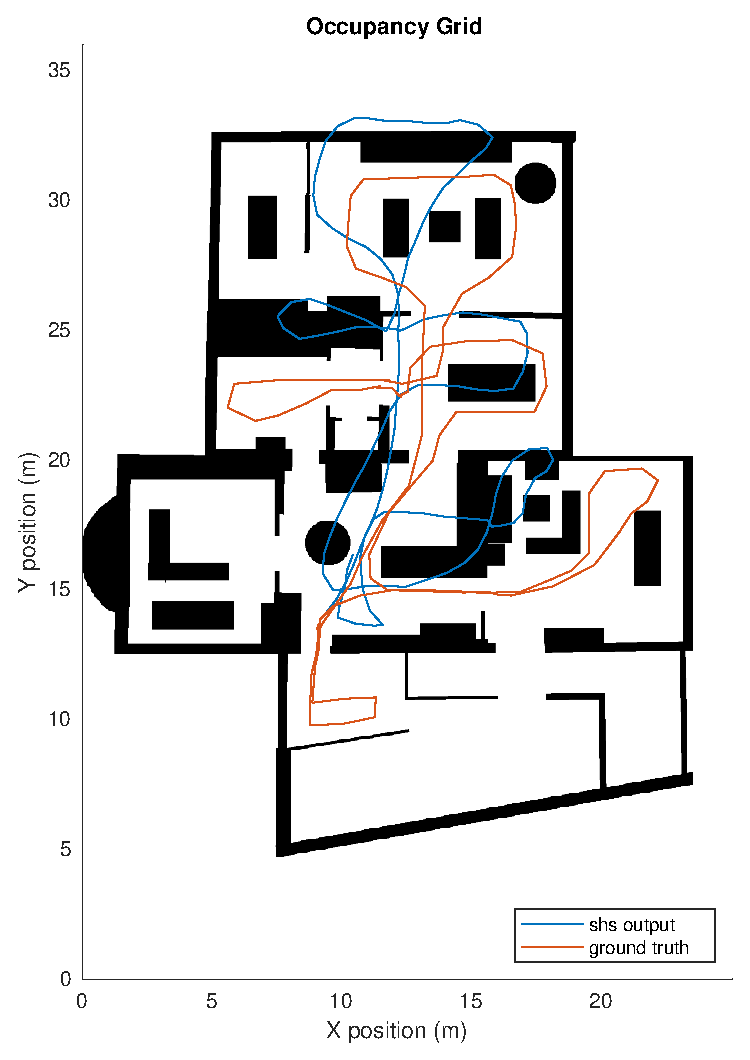
\includegraphics[width=0.9\linewidth]{images/20201029_1042_trial2_shs_1}
		\caption{trajectory comparison}
		\label{fig:trial2_on_map}
	\end{subfigure}
	\begin{subfigure}[t]{.45\textwidth}
		\centering
		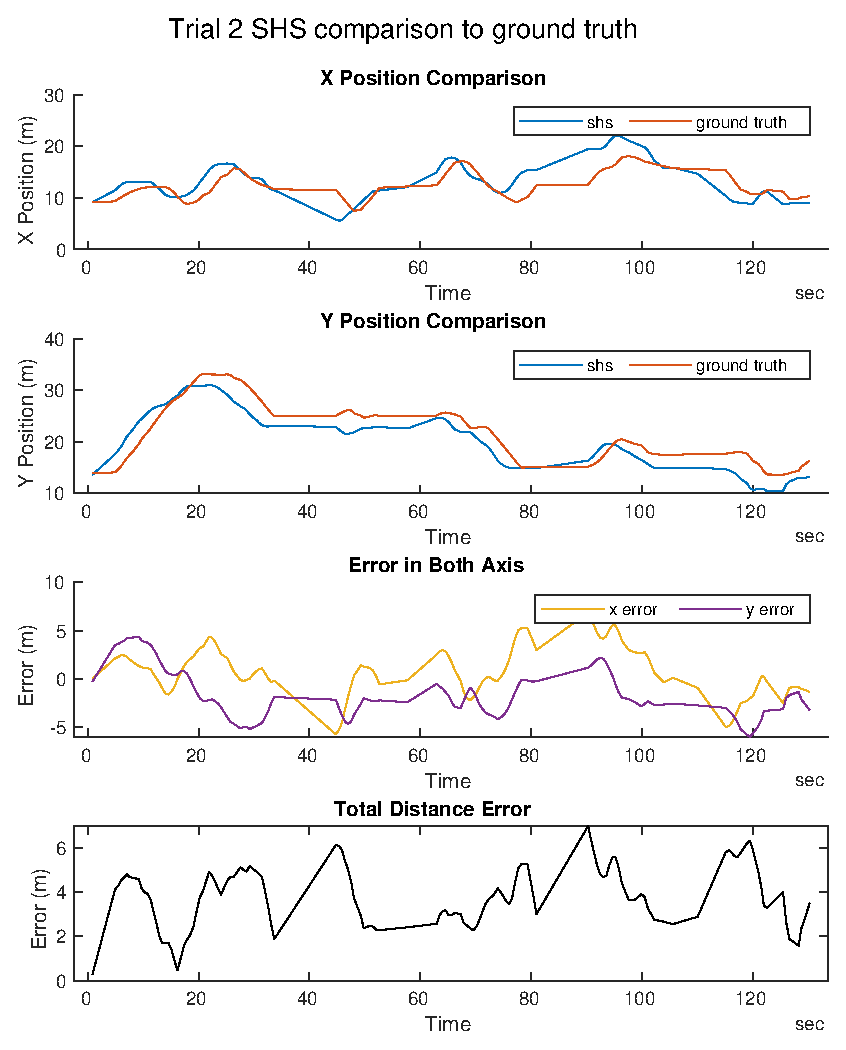
\includegraphics[width=\linewidth]{images/20201029_1042_trial2_shs_2}
		\caption{axis comparison}
		\label{fig:trial2_comparison}
	\end{subfigure}
\setlength{\belowcaptionskip}{-20pt}
	\caption{Qualitative SHS comparison of trial 2 with ground truth}
	\label{fig:trial2_shs_gt_comparison}
\end{figure}

\subsubsection{Trial 3}



%
% Another appendix chapter
\chapter{Yet Another Appendix}


\section{Test Section (Again?)}

Ok, all is well.


%========================== Back matter ======================================
\backmatter
%
% Bibliography
%\bibliographystyle{ieeetr}      % This style puts references in order of appearance
\bibliographystyle{plain}      % This style puts references in alphabetic order
\printbib{MyBib}
%
%
% Glossary
\chapter{Glossary} %
%
\printacronyms
\begin{acronym}[\hspace{0.8in}] % 0.8in is also used by the nomenclature

	\acro{3mE}[3\textlarger{m}E]{Mechanical, Maritime and Materials Engineering}%

	\acro{AMS}{American Mathematical Society}%

	\acro{DCSC}{Delft Center for Systems and Control}%

	\acro{TU}[TU D\textlarger{elft}]{Delft University of Technology}%

	\acro{PDR}{Pedestrian Dead Reckoning}%

	\acro{SHS}{Step and Heading System}%

	\acro{IMU}{Inertial Measurement Unit}%

	\acro{ZUPT}{Zero Velocity Update}%

	\acro{DTW}{Dynamic Time Warping}%

	\acro{NASC}{Normalized Auto-correlation based Step Counting}

	\acro{INS}{Inertial Navigation System}

	\acro{HMM}{Hidden Markov Model}

	\acro{MEMS}{Micro-Electromechanical Systems}

	\acro{COM}{Center of Mass}

	\acro{EKF}{Extended Kalman Filter}

	\acro{PCA}{Principal Component Analysis}

	\acro{FLAM}{Forward and Lateral Accelerations modeling}

	\acro{FIS}{Frequency analysis of Inertial Signals}

	\acro{SLAM}{Simultaneous Localization and Mapping}

	\acro{SVM}{Support Vector Machine}

	\acro{DT}{Decision Tree}

\end{acronym}%
%
%
% Nomenclature
\printnomencl%
%
% Index
\cleardoublepage
\printindex

\end{document}
